\section{Exercise 0: Intro}

The first or zero exercise is quite forward and can bee seen as a warm-up exercise. 
The goal is to get familiar with the tools and the environment and write a small program for a blinking LED (see following code).

\begin{minted}
    [
        frame=lines,
        framesep=2mm,
        baselinestretch=1.2,
        linenos
    ]
    {C}

    const int ledPin =    LED_BUILTIN;  // The onboard LED pin
    const int delayTime = 1000;         // Delay time in milliseconds (1 second)

    void setup() {
      pinMode(ledPin, OUTPUT);
    }

    void loop() {
      digitalWrite(ledPin, HIGH);       // Turn the LED on
      delay(delayTime);
    
      digitalWrite(ledPin, LOW);        // Turn the LED off
      delay(delayTime);
    }
\end{minted}


\section{Exercise 1; Internal RGB}

In the first exercise we are going to use the internal RGB LED to switch between the three colors red, green and blue.
Cause there is also a template for this exercise, we will not go into detail here.

\begin{minted}
    [
        frame=lines,
        framesep=2mm,
        baselinestretch=1.2,
        linenos
    ]
    {C}

    #include <WiFiNINA.h>

    const int delayTime = 500; // Delay time in milliseconds (0.5 seconds)

    void setup() {
      pinMode(LEDR, OUTPUT);
      pinMode(LEDG, OUTPUT);
      pinMode(LEDB, OUTPUT);
    }

    void loop() {
      blink_red();
      delay(delayTime);
      blink_blue();
      delay(delayTime);
      blink_green();
      delay(delayTime);
    }

    void blink_red(){
      Serial.print("Red\n");
      digitalWrite(LEDR, HIGH);   // Red
      digitalWrite(LEDB, LOW);    // Blue
      digitalWrite(LEDG, LOW);    // Green
    }

    void blink_blue(){
      Serial.print("Blue\n");     
      digitalWrite(LEDR, LOW);    // Red
      digitalWrite(LEDB, HIGH);   // Blue
      digitalWrite(LEDG, LOW);    // Green
    }

    void blink_green(){
      Serial.print("Green\n");
      digitalWrite(LEDR, LOW);    // Red
      digitalWrite(LEDB, LOW);    // Blue
      digitalWrite(LEDG, HIGH);   // Green
    }
\end{minted}


\section{Exercise 2: Temperature Sensor}

In the second exercise we are going to use the internal temperature sensor to measure the temperature of the Arduino board.
Also we will use the LEDs from the task before to visualize the temperature like described in the task.
\newline
\newline
The following figures show the different states of the LEDs depending on the temperature.
As it can be seen in the figures, the board was cooled down using a cooling pad and heated up using a hair dryer.
\newline
The code for this exercise can be seen on the github repository \url{https://github.com/Smokey95/AIN_Ubiquitous_Computing/blob/main/exercise/exercise2_temperature/exercise2_temperature.ino}.


\begin{figure}[h!]
    \centering
    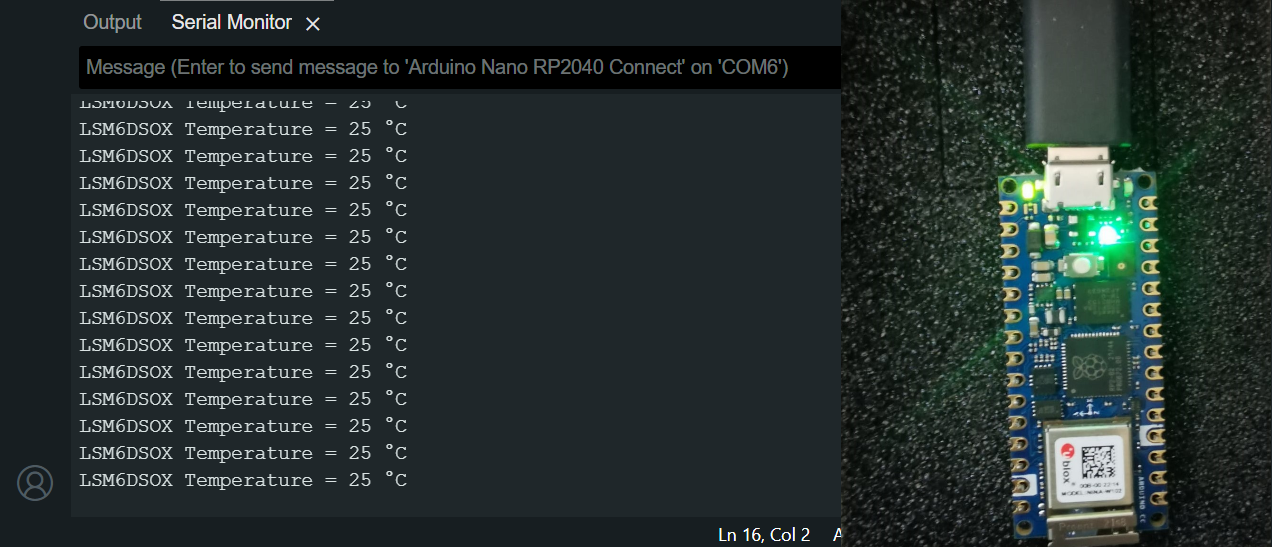
\includegraphics[width=1\textwidth]{exercise_intro/exercise2_temperature_green}
    \caption{Temperature Sensor between 20 and 36 degrees Celsius}
    \label{fig:temperature_sensor_green}
\end{figure}

\begin{figure}[h!]
  \centering
  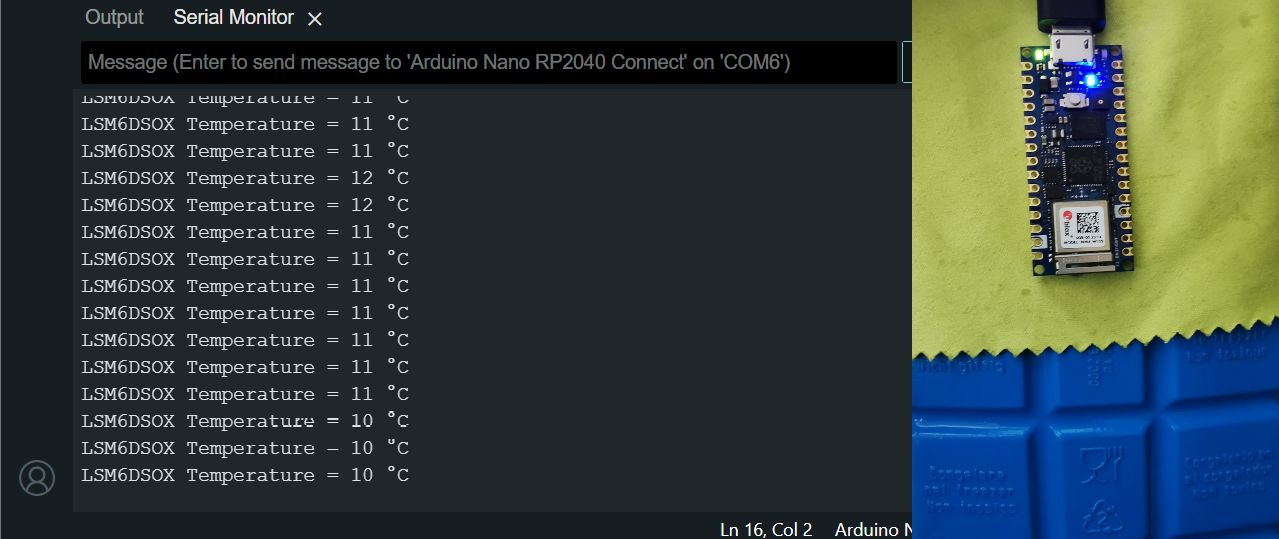
\includegraphics[width=1\textwidth]{exercise_intro/exercise2_temperature_blue}
  \caption{Temperature Sensor under 20 degrees Celsius}
  \label{fig:temperature_sensor_blue}
\end{figure}

\begin{figure}[h!]
  \centering
  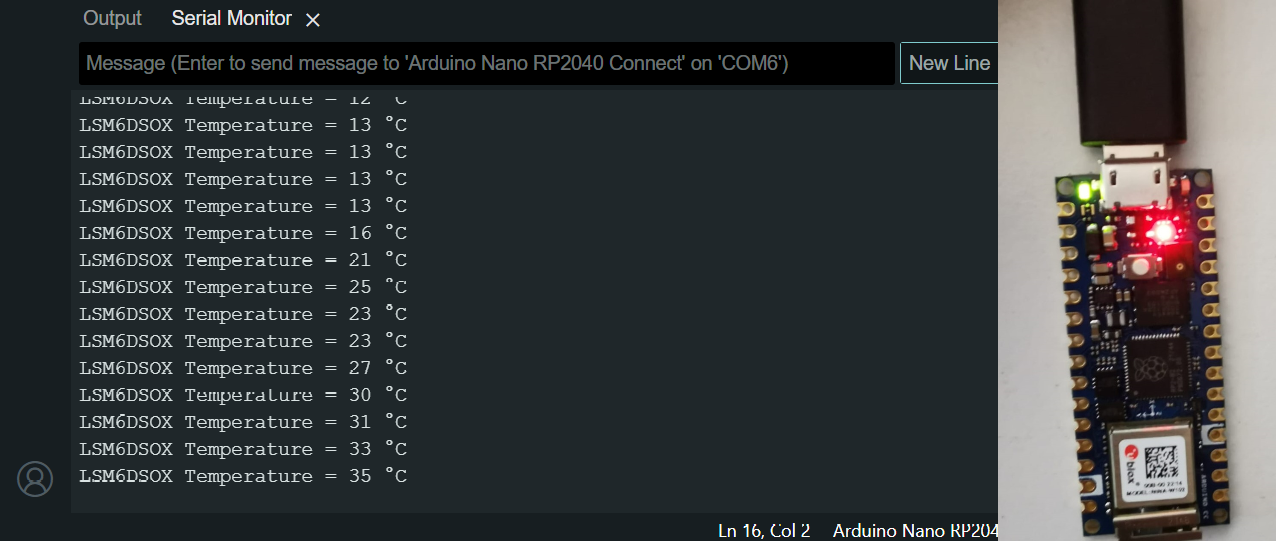
\includegraphics[width=1\textwidth]{exercise_intro/exercise2_temperature_red}
  \caption{Temperature Sensor above 36 degrees Celsius}
  \label{fig:temperature_sensor_red}
\end{figure}

\newpage

\section{Exercise 3: Microphone}

In the third exercise we are going to use the internal microphone to measure the sound level.
Therefore we used the link provided in the task description.
Like seen in the figures below, the LED turn on/off when a certain sound level is reached.
\newline
\newline
Like before the code for this exercise can be seen on the github repository \url{https://github.com/Smokey95/AIN_Ubiquitous_Computing/blob/main/exercise/exercise3_microphone/exercise3_microphone.ino}
It has to be noted that the \code{while-loop} for preventing the program from running till a serial monitor is connected will only work 
if all monitors are closed (even in other Arduino IDE instances).

\begin{figure}[h]
  \centering
  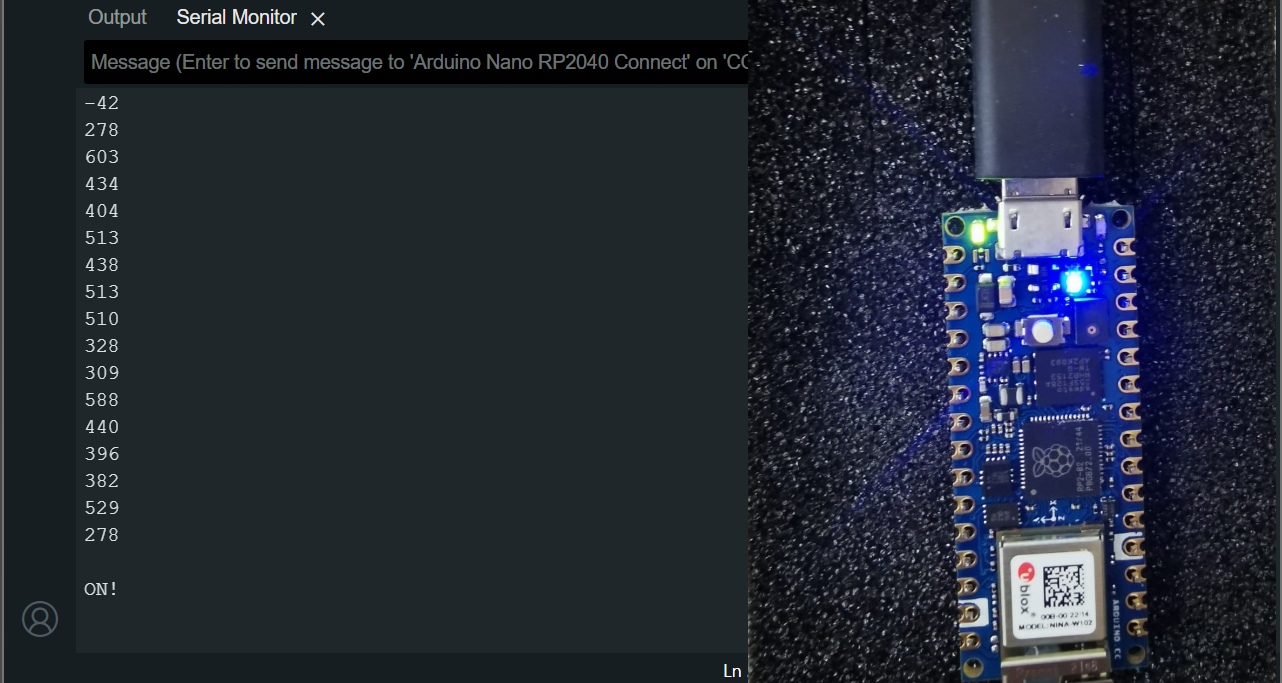
\includegraphics[width=1\textwidth]{exercise_intro/exercise3_mic_on}
  \caption{Sound detected, LED on}
  \label{fig:microphone_on}
\end{figure}

\begin{figure}[h]
  \centering
  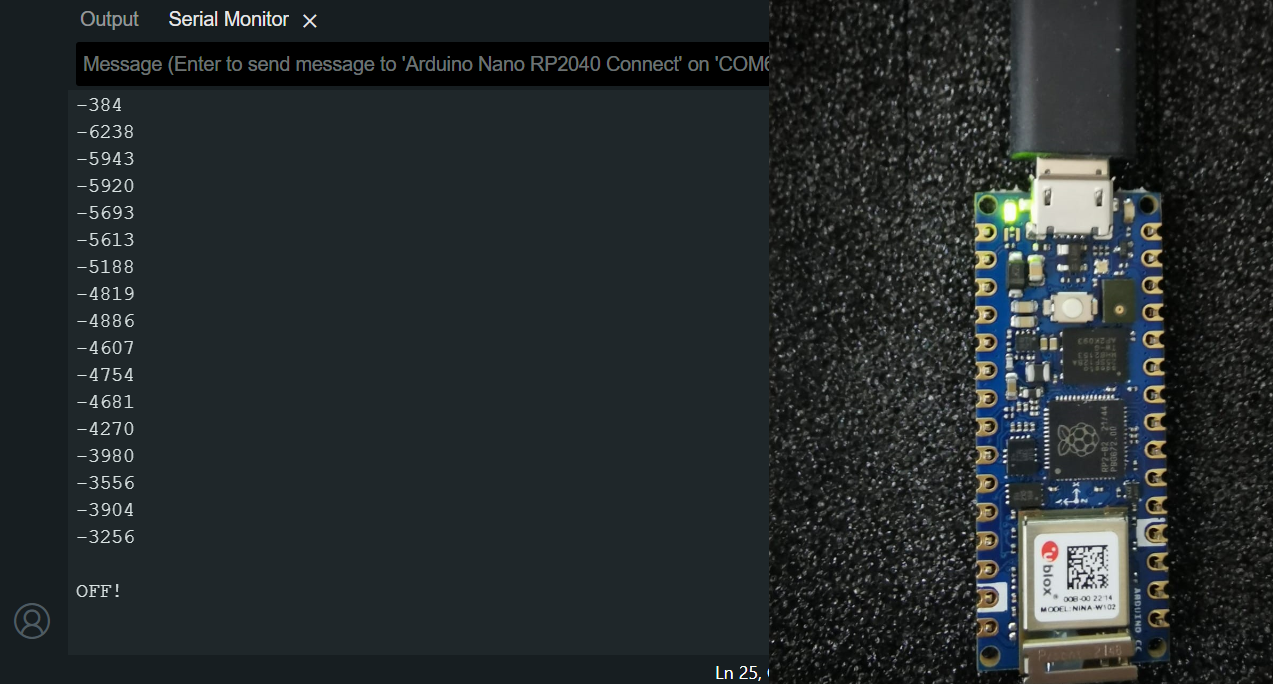
\includegraphics[width=1\textwidth]{exercise_intro/exercise3_mic_off}
  \caption{Sound detected, LED off}
  \label{fig:microphone_off}
\end{figure}


\section{Exercise 4: Posture Detector. Accelerometer}

In the last exercise we are going to use the internal accelerometer to detect the posture of the Arduino board.
Therefore we used the link provided in the task description to realize the following code as well as the serial monitor output seen in figure \ref{posture_detector}.
Like before the code can be seen on the github repository \url{https://github.com/Smokey95/AIN_Ubiquitous_Computing/blob/main/exercise/exercise4_posture/exercise4_posture.ino}.

\begin{figure}[h]
  \centering
  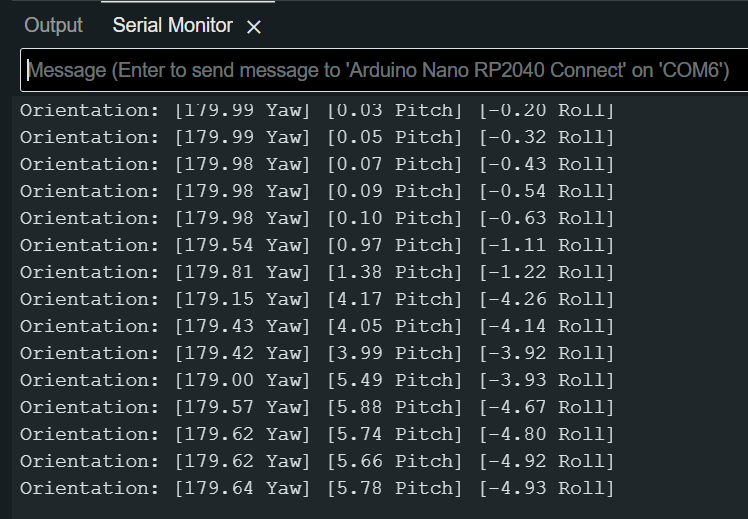
\includegraphics[width=1\textwidth]{exercise_intro/exercise_4_orientation}
  \caption{Posture Detector}
  \label{posture_detector}
\end{figure}